\documentclass[a4paper]{article}
\usepackage[english]{babel}
\usepackage[utf8x]{inputenc}
\usepackage{graphicx}  % graphics with figure-environment
\usepackage{hyperref}
% colors for hyperlinks
% colored borders (false) colored text (true)
\hypersetup{colorlinks=true,citecolor=black,filecolor=black,linkcolor=black,urlcolor=black}
\usepackage{cite}  % bibliograby
% package for header
\usepackage[automark]{scrpage2}
\pagestyle{scrheadings}
\ihead[]{Handwritten character recognition in MPI}
\ohead[]{\today}
\cfoot[]{\pagemark} 
\setheadsepline[122mm]{0.3mm}
\begin{document}
	\title{
	\Huge Handwritten digit recognition
	}
	
	\vspace{2cm}
	
	\author{\Large \href{mailto:stefan.niculae@my.fmi.unibuc.ro}{Stefan Niculae} \and \Large \href{mailto:ionut.ciocoiu@my.fmi.unibuc.ro}{Ionut Ciocoiu}
	\vspace{3cm}}
	
	\date{
	\large Parallel \& Concurrent Programming Lab Report \\
    \vspace{0.2cm}
	\today
	}

	\maketitle
	\setlength{\parindent}{0pt}

\vspace{5cm}
\begin{abstract}
We implement a neural network to classify handwritten digits. The training is done in parallel, using MPI. We provide a comparison for model hyper-parameters and for training time vs number of processes. It achieves great accuracy and fast training time. An interactive demo is also presented



\end{abstract}
	\newpage
	\tableofcontents
	\newpage


\section{Problem statement}
\label{sec:problem}
Given a picture of a handwritten digit, label it accordingly 0 - 9.

\section{Dataset}
\label{sec:dataset}
We demonstrate our model performance on the MNIST database, widely used dataset for training and testing in the field of machine learning. It contains 70 000 examples of labeled handwritten digits. The digits have been size-normalized and centered in a fixed-size image \cite{mnist}. 

\begin{figure}[htb]
\centering

\includegraphics[width=8cm]{images/mnist-images.png}
\caption{Sample MNIST images}
\end{figure}


The images are black-and-white, with a resolution of $28 \times 28$ pixels, represented as an array of $784$ values. Each value ranges from $0$ to $1$ indicating the amount of blackness in the pixel.

\begin{figure}[htb]
\centering
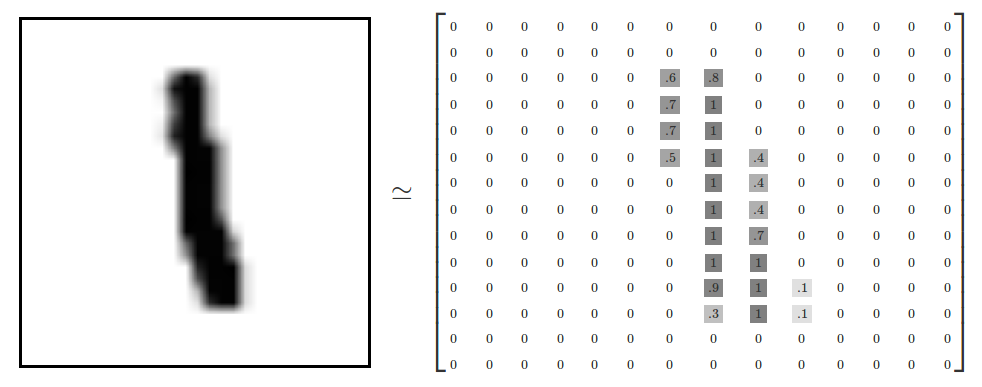
\includegraphics[width=8cm]{images/mnist-matrix.png}
\caption{Matrix representation of a digit}
\end{figure}


\newpage 

\bibliographystyle{ieeetr}
	\bibliography{references} % expects file "references.bib"
	\addcontentsline{toc}{section}{References}
\end{document}
